\documentclass[./main.tex]{subfiles}

\begin{document}
\section{Models}
\label{sec:models}
The following section goes into details with the models from section \ref{sec:model_choice}, that we will also be experimenting with in section \ref{sec:pretraining} and section \ref{sec:finetuning}. The section starts off with section \ref{sec:3DConv}, where we describe the architecture behind the most simple models we will be implementing. Throughout section \ref{sec:bi-ConvLSTMs} we describe the architecture behind the two different bidirectional convolutional LSTMs that we will be experimenting with. This is then followed by section \ref{sec:deciwatch}, where we cover the architecture of our Transformer-based model. Lastly, in section \ref{sec:Mask_RCNN}, we give a brief overview of the already developed keypoint detector.

\subsection{3DConv}
\label{sec:3DConv}
\begin{figure}[htbp]
    \centering
    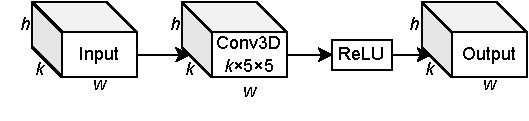
\includegraphics[width=0.8\textwidth]{./entities/baseline.pdf}
    \caption{Illustration of 3DConv.}
    \label{fig:baseline}
\end{figure}

\noindent The first model we will be using is a very simple baseline model based on a 3-dimensional convolution. Throughout this project, we will be refering to this model as \textbf{3DConv}. Figure \ref{fig:baseline} illustrates the architecture of the model.
\\
\\
The model takes a sequence of $T \in \mathbb{N}$ estimated poses $\hat{\mathcal{P}} = \{\hat{\bm{P}}^t\}_{t = 1} ^T$ as input, where each estimated pose $\hat{\bm{P}}^t \in \mathbb{R}^{K \times h \times w}$ is represented using heatmaps, such that $K \in \mathbb{N}$ is the amount of keypoints in each estimated pose, $h \in \mathbb{N}$ is the height of each heatmap and $w \in \mathbb{N}$ is the width of each heatmap.
\\
\\
Once the data has been passed to the model, the processing of the data is very simple. As illustrated in Figure \ref{fig:baseline}, the model starts by applying a 3-dimensional convolutional layer to the input data. The convolutional layer consists of $K \in \mathbb{N}$ filters, each with a kernel-size of $T \times 5 \times 5$. To ensure the input and output of the convolutional layer has the same shape, we pad the input with zeros.
\\
\\
Once the convolutional layer has processed the data, the ReLU activation-function is applied element-wise to the data, resulting in the final prediction of the model.

\subsection{Bidirectional Convolutional LSTM (bi-ConvLSTM)}
\label{sec:bi-ConvLSTMs}
\noindent Our second and third model are based on the LSTM-extension of Unipose-LSTM by Artacho and Savakis \cite{https://doi.org/10.48550/arxiv.2001.08095}. Artacho and Savakis' model was based on a unidirectional convolutional LSTM. However, as we do not require our model to work in real-time, and as we believe a bidirectional convolutional LSTM would be benifical, our models will be based on a bidirectional convolutional LSTM. The major difference between our second and third model is how they combine the information of the two sequence directions.
\\
\\
Both models take a sequence of $T \in \mathbb{N}$ estimated poses $\hat{\mathcal{P}} = \{\hat{\bm{P}}^t\}_{t = 1} ^T$ as input, where each estimated pose $\hat{\bm{P}}^t \in \mathbb{R}^{K \times h \times w}$ is represented as a set of heatmaps, where $K \in \mathbb{N}$ is the amount of keypoints, $h \in \mathbb{N}$ is the height of each heatmap and $w \in \mathbb{N}$ is the width of each heatmap. 

\subsubsection{Model S}
\begin{figure}[htbp]
    \centering
    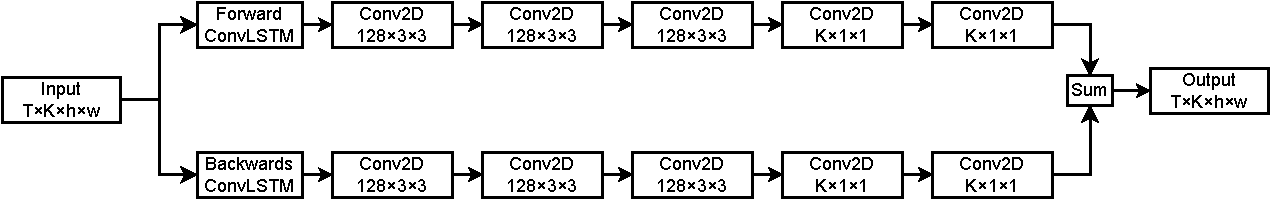
\includegraphics[width=\textwidth]{./entities/bi_conv_lstm.pdf}
    \caption{Illustration of the implemented bidirectional convolutional LSTM, where the two sequence orders are summed together.}
    \label{fig:bi_conv_lstm}
\end{figure}
\noindent Figure \ref{fig:bi_conv_lstm} illustrates the architecture of the second model. We will throughout this project refer to this model as \textbf{bi-ConvLSTM Model S}. The model starts by branching into two seperate branches, that processes the estimated poses in opposite sequence order. Each branch processes the estimated poses one frame at a time. This is done by first applying a convolutional LSTM to the input frame at time step $t \in \mathbb{N}$, using the preceding output of the convolutional LSTM as the hidden state. Each convolutional LSTM is followed by five 2-dimensional convolutional layers, each applying $128$ filters, except for the last convolutional layer of each branch, which aplies $K$ filters. The first three convolutional layers use a kernel size of $3 \times 3$, whereas the following two convolutional layers use a kernel size of $1 \times 1$. The outputs of the two branches are then summed together element-wise.
\\
\\
All convolutional layers use a stride of one and zero-padding on the input, such that the output of each convolutional layer has the same dimensions as the input to the convolutional layer.

\subsubsection{Model C}
\begin{figure}[htbp]
    \centering
    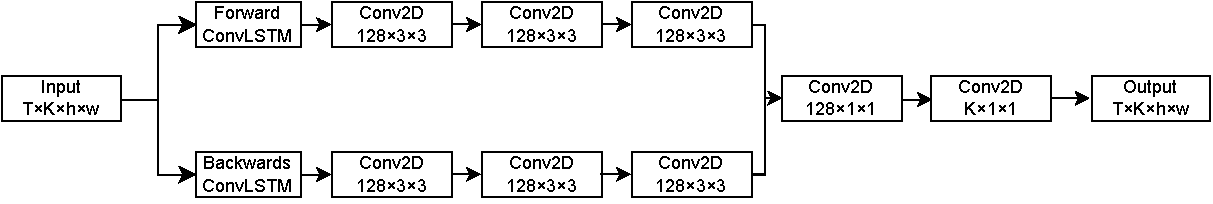
\includegraphics[width=\textwidth]{./entities/unipose2.pdf}
    \caption{Illustration of the implemented bidirectional convolutional LSTM, where the two sequence orders are concatenated together and processed by two convolutional layers.}
    \label{fig:unipose2}
\end{figure}

\noindent Looking at our second model, we see one major problem with the architecture behind it: the model does not have any option of prioritizing one processing order over the other, as the two branches are just summed together. Our third model aims at solving this problem.
\\
\\
Figure \ref{fig:unipose2} illustrates the architecture of our third model. We will through this project refer to this model as \textbf{bi-ConvLSTM Model C}. This model is very similar to the previous model. It also starts off by branching into two seperate branches, that processes the estiamted poses in opposite sequence orders, where each branch processes the estimated poses one frame at a time. Similarly to the previous model, this model also starts off by applying a convolutional LSTM to the input frame, by using the preceding output of the convolutional LSTM as the hidden state. Further, each convolutional LSTM is also fillowed by three 2-dimensional convolutional layers, each applying $128$ filters with a kernel size of $3 \times 3$. 
\\
\\
Different from the previous model, this model concatenates the output of each branch to form a $256 \times h \times w$ tensor, which is then processed by two $1 \times 1$ 2-dimensional convolutional layers with $128$ and $K$ filters, respectively.
\\
\\
Similarly to the second model, all convolutional layers also use a stride of one and zero-padding on the input, such that the output of each convolutional layer has the same dimensions as the input to the convolutional layer.

\subsection{DeciWatch}
\label{sec:deciwatch}
\begin{figure}[htbp]
    \centering
    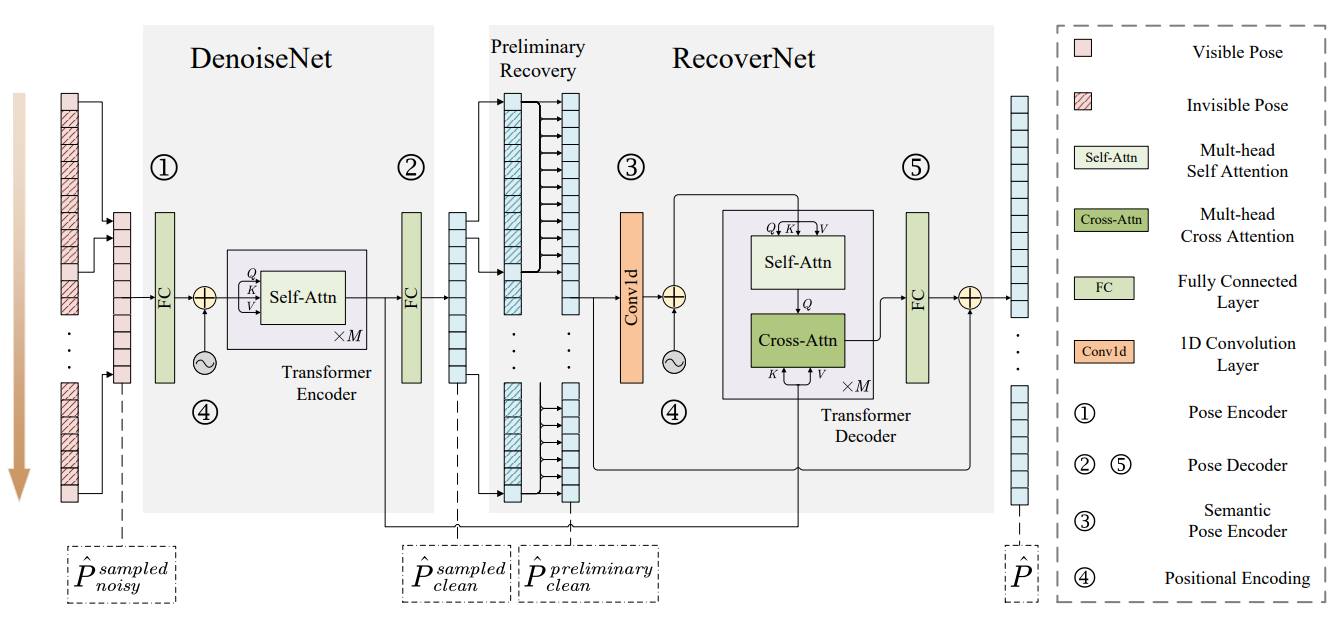
\includegraphics[width=\textwidth]{./entities/deciwatch.PNG}
    \caption{Illustration of the DeciWatch \cite{https://doi.org/10.48550/arxiv.2203.08713}}
    \label{fig:deciwatch}
\end{figure}
\noindent The last model we implement is a transformer-based model named \textit{DeciWatch}, introduced by Zeng \textit{Et al.} \cite{https://doi.org/10.48550/arxiv.2203.08713}, which is illustrated in Figure \ref{fig:deciwatch}. The model works by only processing some of the input-frames. It consists of two parts: the \textit{DenoiseNet} and the \textit{RecoverNet}. The aim of DenoiseNet is to denoise the estimated poses given as input to the model, whereas the aim of RecoverNet is to recover the poses of the missing frames. The following description of the model is based on an interpretation of the official paper behind DeciWatch \cite{https://doi.org/10.48550/arxiv.2203.08713}.
\\
\\
More specifically, the model takes a sequences of $T \in \mathbb{N}$ estimated poses $\hat{\mathcal{P}} = \{\hat{\bm{P}}^t\}_{t = 1} ^T$ as input, where $\hat{\bm{P}}^t$ is represented by a 2-dimensional keypoint position. Due to redundancy in consecutaive frames and continuity of human poses, the model actually do not need all of the frames. Thus, the model starts by sampling every $n$th frame to select sparse poses $\hat{\bm{P}}^{sampled} _{noisy} \in \mathbb{R}^{\frac{T}{n} \times 2K}$, where $K \in \mathbb{N}$ is the number of keypoints. These sampled poses are then passed to DenoiseNet.
\\
\\
The goal of DenoiseNet is to denoise the sparse poses, that were estimated by a single-frame pose estimator. The denoise process can be formulated as
\begin{equation}
    \hat{\bm{F}}_{clean} ^{sampled} = \textbf{TransformerEncoder} \left( \hat{\bm{P}}_{noisy} ^{sampled} \bm{W}_{DE} + \bm{E}_{pos} \right).
\end{equation}
That is, $\hat{\bm{P}}_{noisy} ^{sampled}$ is first encoded through a linear projection matrix $\bm{W}_{DE} \in \mathbb{R}^{2K \times C}$ and summed with a positional embedding $\bm{E}_{pos} \in \mathbb{R}^{\frac{T}{n} \times C}$. This is then passed to a transformer-encoder consisting of $M \in \mathbb{N}$ multi-head Self-Attention blocks, resulting in the noisy poses being embedded into a clean feature $\hat{\bm{F}}_{clean} ^{sampled} \in \mathbb{R}^{\frac{T}{n} \times C}$, where $C \in \mathbb{N}$ is the embedding dimensions. Lastly, another linear projection matrix $\bm{W}_{DD} \in \mathbb{R}^{C \times 2K}$ is used to obtain the denoised sparse poses
\begin{equation}
    \hat{\bm{P}}_{clean} ^{sampled} = \hat{F}_{clean} ^{sampled} \bm{W}_{DD}.
\end{equation}
After the sparse poses has been denoised as $\hat{\bm{P}}_{clean} ^{sampled} \in \mathbb{R}^{\frac{T}{n} \times 2K}$, the data is passed to the RecoverNet, whose goal is to recover the absent poses. First, a linear transformation $\bm{W}_{PR} \in \mathbb{R}^{T \times \frac{T}{n}}$ is applied to perform preliminary sequence recovery to get $\hat{\bm{P}}_{clean} ^{preliminary} \in \mathbb{R}^{T \times 2K}$ by
\begin{equation}
    \hat{\bm{P}}_{clean} ^{preliminary} = \bm{W}_{PR} \hat{\bm{P}}_{clean} ^{sampled}.
\end{equation}
To improve the recovery of the absent poses a transformer-decoder and positional embedding is used together with a 1D convolutional layer to bring temporal semantics into pose encoding to encode the neighboring $D \in \mathbb{R}$ frames' poses into pose tokens. Thus, RecoverNet, and the final prediction of DeciWatch, can be summarized by
\begin{equation}
    \hat{\bm{P}} = \textbf{TransformerDecoder}\left(Conv1d \left( \hat{\bm{P}}_{clean} ^{preliminary} \right) + \bm{E}_pos, \hat{\bm{F}}_{clean} ^{sampled} \right)\bm{W}_{RD} + \hat{\bm{P}}_{clean} ^{preliminary}
\end{equation}
where $\bm{W}_{RD} \in \mathbb{R}^{C \times 2K}$ is another linear transformation layer. Further, as illustrated by Figure \ref{fig:deciwatch}, key information is drawn in the the Cross-Attention block by leveraging the denoised features $\hat{\bm{F}}_{clean} ^{sampled}$.
\\
\\
To avoid overfitting, dropout is applied to the input of each sub-layer and sums of the embeddings of the transformer-encoder and transformer-decoder, as well as to the positional encodings.

\subsection{Mask R-CNN for Human Pose Estimation}
\label{sec:Mask_RCNN}
The last model we will be using is the \textit{Mask R-CNN for human pose estimation} as introduced by He \textit{Et al.} in 2017 \cite{https://doi.org/10.48550/arxiv.1703.06870}. Unlike the previously described model, we will not be implementing this model, but instead use an already  developed model on the ClimbAlong dataset, which has been provided by ClimbAlong A/S. As we will not be implementing this model, we will here not go into the details of how the model works, but instead just give a brief overview of the model. We will throughout this project be refering to this already developed model as the \textbf{keypoint detector}.
\\
\\
The model takes a single rgb-image with height $h_{in} \in \mathbb{N}$ and width $w_{in} \in \mathbb{N}$ as input and returns $K \in \mathbb{N}$ heatmaps of height $h_{out} \in \mathbb{N}$ and width $w_{out} \in \mathbb{N}$ such that each heatmap corresponds to a single keypoint where the position of the element with the greatest value corresponds is the location of the predicted keypoint. The Mask R-CNN by ClimbAlong A/S uses $h_{out} = w_{out} = 56$ and $K = 25$.
\\
\\
Each heatmap corresponds to the predicted bounding-box of the person that the keypoints corresponds to. Further, this bounding-box has been resized such that it is squared, discarding the aspect ratio of the original bounding-box.

\end{document}